\chapter{Grundlagen}

In diesem Kapitel wird das Wissen vermittelt, welches benötigt wird, um zu verstehen, wie \acp{NNUE} im Rahmen von Schachcomputern funktionieren. Zuerst wird die Evaluation, wie sie in herkömmlichen Schachcomputern funktioniert, erklärt, auch \ac{HCE} genannt. Weiterhin wird auf die grundlegenden Bestandteile, die für überwacht lernende \acp{FNN} von Bedeutung sind, eingegangen. Außerdem wird erläutert, was \ac{SIMD} ist und wie diese Vektoroperationen in C/C++ verwendet werden. Zuletzt wird die grundlegende Funktionsweise von \acp{NNUE} vermittelt, die auf den davor gelegten Grundsteinen aufbaut.

\section{Hand-Crafted Evaluation}
\label{chap:HCE}

Es ist wichtig zu wissen, wie die \ac{HCE} eines Schachcomputers funktioniert, da sie nicht nur die Variante ist, die in jedem starken Schachcomputer vor 2017 eingesetzt wurde, sondern auch heute noch in Kombination mit \ac{NNUE} eingesetzt wird. Bei \ac{NNUE}-Schachcomputern wird sie oft in Kombination mit der \ac{NN}-Evaluation genutzt, weil sie besser in extremen Stellungen funktioniert. Besitzt beispielsweise Weiß in einer Position eine Dame mehr, muss nicht die teurere Berechnung des \acp{NNUE} durchgeführt werden, um zu entscheiden, dass Weiß im Vorteil ist.

Die \ac{HCE} einer Schachposition ist eine heuristische Methode der Position einen numerischen Wert zuzuordnen. Vor der Verbreitung von \acp{NN} war \ac{HCE} die einzige Form der Positions-Evaluation. Gäbe es unendliche Ressourcen, könnten aus jeder Position alle möglichen Zugfolgen per Brute Force bestimmt und den Positionen einer der drei Werte: -1 (Verlust), 0 (Remis), 1 (Gewinn) gegeben werden. In der Realität ist es nicht möglich, den exakten Wert der Stellung zu kennen. Deshalb wird in der \ac{HCE} versucht, anhand von Menschen festgelegten Kriterien der Position einen Wert zuzuordnen. Die so gewonnene Bewertung wird in der Zugsuche verwendet, um den besten Zug, abhängig von den per Hand gewählten Kriterien, zu finden. Die Evaluation wird aus Sicht der Seite, die gerade am Zug ist, angegeben. Das ist wichtig für den verwendeten Suchalgorithmus (Alpha-Beta-Suche) \cite{Slagle1969}.

Die \ac{HCE} eines Schachcomputers ähnelt in einigen Aspekten mehr einer Philosophie als einer Funktion. Schach ist ein Spiel, das es seit über 1000 Jahren gibt. In dieser Zeit haben Menschen Regeln überlegt, um besser Schach zu spielen. All diese Regeln in die Evaluationsfunktion zu integrieren, ist nicht ratsam. Es ist ein Abwägen zwischen Wissen und Geschwindigkeit. Je mehr Regeln dem Computer gegeben werden, umso weniger weit kann er vorausschauen.

Wenn ein Mensch Schach spielen lernt, ist der Wert der Figuren eines der ersten Erkenntnisse. Das ist ebenfalls der wichtigste Faktor für einen Schachcomputer, wie schon \citeauthor{Shannon1950} \citeyear{Shannon1950} \cite{Shannon1950} erkannte. Die Angabe der Materialwertung wird bei Computern als \ac{CP} angegeben, um so mehr Spielraum für feingranulare Faktoren zu lassen. Figuren werden ebenfalls anhand ihrer Position bewertet. Dafür gibt es sogenannte Piece Square Tables, die jeder Figur abhängig von ihrer Position einen Wert zuordnen. Beispielsweise ist ein Springer am Rand des Brettes deutlich weniger wert als einer im Zentrum, auch bekannt als \enquote{ein Springer am Rand bringt Kummer und Schand}. Weitere nennenswerte Aspekte der \ac{HCE} sind die Mobilität und Schwachstellen \cite[S. 228]{Levy1988}.

% weitere evlauations aspekte: Mobilität und Schwachstellen
Mobilität beschreibt die Beweglichkeit der Figuren. Sie kann aus der Anzahl der Felder, auf die eine Figur ziehen kann, berechnet werden. Das ist unbrauchbar, weil unbeschützte Felder und die Felder gefesselter Figuren nicht Teil der Mobilität sein sollten \cite[S. 228]{Levy1988}. Mit Schwachstellen sind ungeschützte Figuren, die Sicherheit des Königs, Probleme in der Bauernstruktur und Figuren, die höherwertige Figuren angreifen, gemeint \cite[S. 228]{Levy1988}.

% erklären warum verschiedene Spielphasen eine Rolle spielen
Viele der \ac{HCE}-Aspekte profitieren von einer Differenzierung verschiedener Spielphasen. Schach lässt sich in drei Spielphasen teilen: die Eröffnung, das Mittelspiel und das Endspiel \cite[S. 8]{Levy1988}. Beispielsweise ist es sinnvoll, den Wert der Figuren an die aktuelle Spielphase anzupassen. Ein Bauer im Endspiel ist mehr wert als in der Eröffnung. Zwischen den verschiedenen Phasen wird meist durch die Anzahl der Figuren unterschieden. Da zwischen zwei ähnlichen Stellungen, die in zwei unterschiedlichen Phasen sind, kein großer Unterschied durch den Phasenwechsel entsteht, ist es sinnvoll einen Wert für beide Phasen zu berechnen und dazwischen zu interpolieren.

\section{Neuronale Netze}

\Acp{KNN}, oder einfach \acp{NN} genannt, sind Computersysteme, die dem biologischen Vorbild des Gehirns nachempfunden sind. Analog zu seinem biologischen Vorbild besteht ein \ac{NN} aus Neuronen, die miteinander vernetzt sind. Jedes Neuron reagiert auf eingehende Signale mit einer bestimmten Ausgabe. Diese Ausgabe kann sich durch neu gewonnene Erfahrungen anpassen und ermöglicht, zukünftig besser zu reagieren.

% erklären wie der generelle Aufbau ist
In \autoref{fig:beispiel-nn} ist ein einfaches \Acl{NN} zu sehen. Es besteht aus drei Schichten. Die erste Schicht, die Eingabeschicht, nimmt Eingabedaten entgegen. Eingabedaten können ganz unterschiedliche Daten repräsentieren. Ist der Eingabedatensatz beispielsweise ein 100 × 100 Schwarz-Weiß-Bild, ist dies eine Möglichkeit die Eingaben darzustellen. Die Eingabeschicht besteht dann aus 1000 Neuronen, die pro Neuron den Zustand eines Pixels (0 = Weiß, 1 = Schwarz) des Bildes gefüttert bekommen. Die zweite Schicht heißt versteckte Schicht, weil von außen nur die Eingabedaten und das Ergebnis sichtbar ist. Sie empfängt die Informationen der Eingabeschicht, gewichtet sie und gibt sie an die Ausgabeschicht weiter. Die versteckte Schicht kann aus mehreren Schichten bestehen. Ein \ac{NN} mit mehr als drei versteckten Schichten heißt \ac{DNN}. Die letzte Sicht, die Ausgabeschicht, spiegelt das Ergebnis des \acp{NN} wider. Ein Netz, das versucht Bilder zwischen Hunden und Katzen zu unterscheiden, kann zwei Ausgabeneuronen enthalten, eins für die Wahrscheinlichkeit, dass auf dem gegebenen Bild ein Hund ist und eins für die Wahrscheinlichkeit, dass es eine Katze ist. Ein \ac{NN} kann auch nur ein Ausgabeneuron besitzen, wie \zb{} bei der Evaluation einer Schachposition nötig ist. Die Verbindungen der einzelnen Neuronen stellen deren Zusammenhang dar. Wie stark die Abhängigkeit ist, wird durch Gewichte definiert \cite[S. 2--7]{krawczak2013multilayer}.
% Auswahl der Inputdatenspalten gibt an, wieviele Inputneuronen es gibt, die Anzahl der hidden Neuronen ist "egal" je mehr -> desto besser kann das neuronale Netz lernen kinda, output Neuronen gibt die Anzahl der Klassifikationen an, kann auch nur eins sein (regession)

\begin{figure}
  \centering
  % inspired by: https://tex.stackexchange.com/questions/153957/drawing-neural-network-with-tikz
  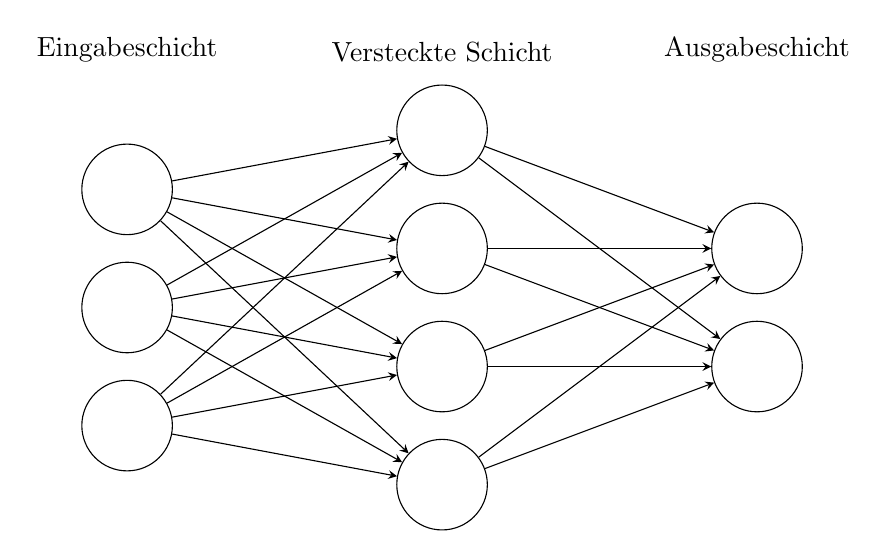
\begin{tikzpicture}[x=2cm, y=1.5cm, >=stealth]
    \tikzstyle{neuron}=[draw,shape=circle,minimum size=1.15cm]
    % draw nerons
    \foreach \m/\l [count=\y] in {1,2,3}
    \node [neuron] (input-\m) at (0,2-\y) {};

    \foreach \m [count=\y] in {1,2,3,4}
    \node [neuron] (hidden-\m) at (2,2.5-\y) {};

    \foreach \m [count=\y] in {1,2}
    \node [neuron] (output-\m) at (4,1.5-\y) {};
    % draw lines  
    \foreach \i in {1,2,3}
    \foreach \j in {1,2,3,4}
    \draw [->] (input-\i) -- (hidden-\j);

    \foreach \i in {1,2,3,4}
    \foreach \j in {1,2}
    \draw [->] (hidden-\i) -- (output-\j);

    \foreach \l [count=\x from 0] in {Eingabeschicht, Versteckte Schicht, Ausgabeschicht}
    \node [align=center, above] at (\x*2,2) {\l};
  \end{tikzpicture}
  \caption{Ein einfaches \acl{NN}. Jedes Neuron einer Schicht ist in Pfeilrichtung mit allen Neuronen der nächsten Schicht vernetzt. Die Verbindungen symbolisieren Gewichte. In den Neuronen werden die eingehenden Gewichte aufsummiert und über eine Transferfunktion zu einem Ausgabewert abgebildet.}
  \label{fig:beispiel-nn}
\end{figure}

Es gibt verschiedene Modelle neuronaler Netze. Für diese Thesis sind lediglich \aclp{FNN} relevant. \acp{FNN} basieren auf dem von \citeauthor{rosenblatt1958perceptron} \cite{rosenblatt1958perceptron} beschriebenen mehrlagigen Perzeptron. Das \ac{FNN} zeichnet sich durch seinen zyklenfreien Aufbau aus. Der Datenfluss führt immer von der Eingabeschicht zur Ausgabeschicht. Das \ac{FNN} gilt als die einfachste Netzwerkarchitektur \cite{Schmidhuber2015}.

In der Praxis, so auch in dieser Arbeit, werden für die Entwicklung Neuronaler Netze Frameworks verwendet. Sie abstrahieren große Teile der Komplexität. Trotzdem ist es wichtig, ihre Funktionsweise zu kennen, um Entscheidungen treffen und Probleme beheben zu können. In den folgenden Unterabschnitten wird grundlegend auf die Einzelteile Neuronaler Netze eingegangen. Zuerst wird das Neuron beschrieben und wie sich seine Aktivität berechnen lässt. Das Unterkapitel Backpropagation beschreibt, wie \acp{NN} lernen.

\subsection{Das Neuron}
\label{chap:neuron}

% Neuronen wie sie im Nervensystems eines Menschen vorhanden sind
Das Neuron ist der elementare Bestandteil eines \acp{NN}. Es wurde \citeyear{McCulloch1943} von \citeauthor{McCulloch1943} \cite{McCulloch1943} eingeführt. Neuronen sind in einem \ac{NN} mit anderen Neuronen verbunden und bilden so beliebig komplexe Funktionen ab. In \autoref{fig:neuron} ist ein einzelnes Neuron zu sehen. Die Eingänge $x_{0}$ bis $x_{n}$ werden mit den Gewichten $w_{0}$ bis $w_{n}$ multipliziert, aufsummiert und mit der Aktivierungsfunktion $f(\varphi)$ aktiviert. Für gewöhnlich ist immer $x_{0}=1$, was ihn zu dem Bias des Neurons mit $w_{0}=b$ macht. Das bedeutet, dass es nur $n$ tatsächliche Eingabewerte gibt: von $x_{1}$ bis $x_{n}$. Konkret lässt sich die Aktivität eines Neurons mit der \autoref{equation:NeuronActivation} und die Ausgabe $y$ mit der \autoref{equation:NeuronOutput} bestimmen:

% mathematische Grundlage für das Neuron und Neuronale Netz
\begin{equation}
  f(\varphi) = \varphi(\sum_{i=0}^{n}w_{i}x_{i})
  \label{equation:NeuronActivation}
\end{equation}

\begin{equation}
  y = f(\varphi)
  \label{equation:NeuronOutput}
\end{equation}

\begin{figure}
  \centering
  % inspired by: https://davidstutz.de/illustrating-convolutional-neural-networks-in-latex-with-tikz/
  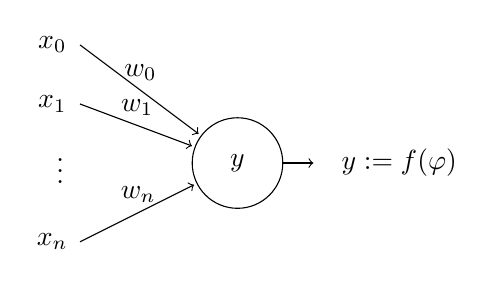
\begin{tikzpicture}[shorten >=1pt,->]
    \tikzstyle{unit}=[draw,shape=circle,minimum size=1.15cm]

    \node[unit](p) at (2,1){$y$};
    \node(dots) at (-0.25,1){\vdots};

    \draw (0,2.5) node[xshift=-10]{$x_0$} -- node [midway,above] {$w_{0}$} (p);
    \draw (0,1.75) node[xshift=-10]{$x_1$} -- node [midway,above] {$w_{1}$} (p);
    \draw (0,0) node[xshift=-10]{$x_n$} -- node [midway,above] {$w_{n}$} (p);
    \draw (p) -- (3,1) node[xshift=30]{$y := f(\varphi)$};
  \end{tikzpicture}
  \caption{Ein einzelnes Neuron mit seinen Eingabe- und Ausgabekomponenten. Die Eingabewerte $x$ werden mit den Gewichten $w$ multipliziert und im Neuron aufsummiert. Anschließend werden sie mit der Transferfunktion $f(\varphi)$ auf einen Ausgabewert abgebildet.}
  \label{fig:neuron}
\end{figure}

% activation functions: linear vs non linear -> linear Functions sorgen dafür, dass nur ein hidden Layer sinnvoll ist, mehrere hidden Layer mit linearen Aktivierungsfunktionen geben keinen Sinn, da sie zu einer Schicht vereinfacht werden können. Deshalb sind nicht-lineare Transferfunktionen interessant, sie ermöglichen es, komplexere Funktionen zu lernen
Die Aktivierungsfunktion, oder auch Transferfunktion, eines Neurons kann linear oder nicht linear sein. Ist die Transferfunktion linear, ergibt ein mehrschichtiges \ac{NN} keinen Sinn, da sie zu einer Schicht vereinfacht werden kann. Außerdem sind lineare \acp{NN} nicht in der Lage, nicht lineare Probleme zu lösen \cite{minsky1969perceptron}. Nicht lineare Transferfunktionen sind interessanter, da sie für nicht lineare Probleme Antworten liefern.

% eingehen auf clipped relu und sigmoid Aktivation Functions
In \autoref{fig:activationfunction} sind zwei Aktivierungsfunktionen zu sehen. In \autoref{fig:sigmoid} ist eine Standardsigmoide abgebildet. Sie sorgt dafür, dass die Ausgabe des Neurons immer zwischen null und eins ist. Berechnet wird sie mit \autoref{equation:sigmoid}. \autoref{fig:Relu} zeigt eine \ac{ReLU}-Transferfunktion. Der niedrigste Wert ist mindestens null. Konkret ist die Berechnung in \autoref{equation:ReLU} angegeben. \ac{ReLU} geht bis ins Unendliche. Wegen der aggressiven Quantisierung wird der Bereich der Aktivierungsfunktionen ebenfalls nach oben begrenzt, auch Clipped\ac{ReLU} (siehe \autoref{equation:ClippedReLU}) genannt \cite{StockfishNNUE}.

\begin{equation}
  Sigmoid(x)=\frac{1}{(1+e^{-x})}
  \label{equation:sigmoid}
\end{equation}

\begin{equation}
  ReLU(x)=max(0,x)
  \label{equation:ReLU}
\end{equation}

\begin{equation}
  ClippedReLU(x)=min(max(0,x),1)
  \label{equation:ClippedReLU}
\end{equation}

\begin{figure}
  \centering
  \begin{subfigure}[t]{.49\textwidth}
    \centering
    \resizebox{.9\textwidth}{!}{%
      \begin{tikzpicture}[declare function={sigma(\x)=1/(1+exp(-\x));}]
        \begin{axis}%
          [
            grid=none,
            xmin=-6,
            xmax=6,
            axis x line=bottom,
            ytick={0,.5,1},
            ymax=1,
            axis y line=middle,
            samples=100,
            domain=-6:6,
            legend style={at={(1,0.9)}}
          ]
          \addplot[blue,mark=none]   (x,{sigma(x)});
        \end{axis}
      \end{tikzpicture}
    }
    \caption{Standardsigmoide Aktivierungsfunktion. Sie ist konvex für Werte unter einem bestimmten Punkt und konkav für Werte darüber. Hier ist dieser Punkt 0. Außerdem nähern sich die Extreme der Funktion den Grenzwerten 0 und 1.}
    \label{fig:sigmoid}
  \end{subfigure}%
  \hfill%
  \begin{subfigure}[t]{.49\textwidth}
    \centering
    \resizebox{.9\textwidth}{!}{%
      \begin{tikzpicture}[declare function={relu(\x)=max(0,\x);}]
        \begin{axis}%
          [
            grid=none,
            xmin=-3,
            xmax=3,
            axis x line=bottom,
            ytick={0,1,2,3},
            ymax=3,
            axis y line=middle,
            samples=1000,
            domain=-3:3,
            legend style={at={(1,0.9)}}
          ]
          \addplot[blue,mark=none]   (x,{relu(x)});
        \end{axis}
      \end{tikzpicture}
    }
    \caption{Rectified linear Aktivierungsfunktion. Die Ausgabe der Funktion beträgt immer mindestens den Wert null und ist sonst linear.}
    \label{fig:Relu}
  \end{subfigure}
  \caption{Beispiele für Aktivierungsfunktionen}
  \label{fig:activationfunction}
\end{figure}

\subsection{Backpropagation und Gradientenabstieg}
\label{chap:bpGradient}
% viel muss man davon nicht kennen, da Pytorch das übernimmt (automatic through automatic differentiation)
Das Besondere an \acp{NN} ist, dass sie lernen, also nach und nach besser werden. Für gewöhnlich wird erwartet, dass ein Programm bei identischer Eingabe immer dasselbe Ergebnis liefert. Ein \ac{NN} hingegen lernt während seiner Trainingsphase aus Fehlern. Es gilt, den Fehler zu minimieren. Dabei handelt es sich um ein Optimierungsproblem. Als Lösung dafür wird der Gradientenabstieg verwendet. Es gibt dafür auch andere Methoden, auf die hier nicht weiter eingegangen wird \cite{StockfishNNUE}.

Der Gradientenabstieg minimiert den Fehler, indem er dem negativen Gradienten einer Verlustfunktion folgt \cite{Ruder2016}. Die Annahme ist, dass die Richtung des Gradienten einer Funktion diese maximiert. Deshalb führt ein Schritt in die entgegengesetzte Richtung zu einer Minimierung der Funktion, also einer Minimierung des Fehlers. Die Lernrate steuert die Schrittweite, die dem negativen Gradienten folgt. Sind die Schritte zu groß, wird das (lokale) Minimum übersprungen. Sind sie klein, dauert die Konvertierung länger oder bleibt in einem lokalen Minimum hängen. Um beide dieser Probleme bestmöglich zu vermeiden, ist die Lernrate nicht konstant, sondern ändert sich über den Trainingszeitraum.

Die Lernrate kann entweder abhängig durch einen festen Plan oder durch ein adaptives Modell angepasst werden. Ein Beispiel für eine fest geplante Änderung ist die Multiplikation der Lernrate mit einem Faktor $x$ alle $n$ Epochen. Eine Epoche ist normalerweise ein Durchgang des gesamten Eingabedatensatzes. Alternativ gibt es verschiedene adaptive Lernraten-Modelle. In dieser Arbeit wird \zb{} Adadelta verwendet. Adadelta ist eine Adaption des Gradientenabstiegs. Diese Variante erweitert den Gradientenabstieg um eine dynamische Lernrate, die akkumulierende Gradienten durch ein Fenster löst. In dem Fenster wird nur die Summe der letzten Gradienten, bestimmt durch eine feste Größe, akkumuliert \cite{Zeiler2012}. Adadelta zeigt gute Leistungen im Vergleich zu anderen adaptiven Lernraten-Modellen und eliminiert das Problem, eine passende Lernrate zu finden.
% vl mal: https://github.com/lucidrains/Adan-pytorch probieren

Es gibt drei Varianten des Gradientenabstiegs \cite{Ruder2016}:
\begin{itemize}
  \item \emph{Batch Gradientenabstieg}, berechnet den Gradienten der gesamten Verlustfunktion über den gesamten Trainingsdatensatz. 
  \item \emph{Stochastischer Gradientenabstieg}, berechnet den Gradienten für jedes Trainingsbeispiel einzeln.
  \item \emph{Mini-batch Gradientenabstieg}, berechnet den Gradienten für jedes Subset der Größe $n$ der Trainingsbeispiele.
\end{itemize}

Die vorherigen Absätze erklären, wie der Fehler durch einen Gradientenabstieg minimiert werden kann. In \autoref{chap:neuron} wird gezeigt, wie die Eingaben und Gewichte eines Neurons zu einem Ergebnis führen. Nun stellt sich die Frage: Welche Werte müssen die Gewichte haben, um den Fehler zu minimieren? Die perfekten Gewichte eines \acp{NN} lassen sich nicht berechnen. Dafür ist die Anzahl der Faktoren zu groß.

Als Backpropagation wird das Verfahren der Fehlerrückführung beschrieben. Es gehört zu der Familie der überwachten Lernverfahren. Damit wird der negative Gradient der Verlustfunktion rückwärts durch das Netz geführt. Dabei werden die Werte der Gewichte angepasst \cite{Wythoff1993}. Die Gewichte werden mithilfe der rekursiven Anwendung der Kettenregel aus der Infinitesimalrechnung und Berechnung einer Ableitung der Unterfunktion einer bekannten übergeordneten Funktion angepasst.

% Die delta lern regel

% the forward pass gives you the error and the backpropagation computes the gradiants and based on the gradiants the optimization algorithm ajusts the weights, the learing rate is the speed at witch changes occure

% \subsection{Convolutional Neural Networks}
% kann vl entfernt werden (schau am ende ob man es noch braucht (seiten))
% nur ein kurzer exkurs da es in andern neuronalen netzen für schach computer verwendet wird

\subsection{Verlustfunktion}

Da ein \ac{NN} aus seinen Fehlern lernen kann, muss ermittelt werden, ob das Netz mit seiner Vorhersage richtig liegt. Mit der Verlustfunktion wird der Fehler an einem bestimmten Punkt der zu bestimmenden Funktion ermittelt. Dafür wird ein Satz von Eingabedaten genommen und dem Netz gegeben, welches eine Vorhersage für eine Ausgabe abhängig von den Gewichten trifft. Diese Ausgabe wird mit dem vorher definierten zu erwartenden Ergebnis verglichen. Basierend darauf wird der Gradient der Verlustfunktion berechnet, der von den in \autoref{chap:bpGradient} beschriebenen Methoden zur Anpassung der Gewichte verwendet wird. In folgendem Text sind zwei Verlustfunktionen beschrieben, die häufig in \acp{NN} eingesetzt werden.

% quadratischer Fehler mit Formel (squared error)
Die mittlere quadratische Fehler-Verlustfunktion ist eine simple Verlustfunktion. Sie nimmt die Summe der quadratischen Differenz der vorhergesagten Werte $y$ mit den Zielwerten $t$ über eine Menge von $n$ Eingabewerten. Das Ergebnis ist eine quadratische Funktion, dessen Gradienten sich gut für Gradientenabstieg eignet. Die entsprechende Funktion ist in \autoref{equation:mse} zu sehen.

\begin{equation}
  MSE(y, t) = \frac{1}{n}*\sum^{n}_{i=1}(y_{i}-t{i})^{2}
  \label{equation:mse}
\end{equation}

% Kreuzentropie
Die Kreuzentropie-Verlustfunktion eignet sich für Klassifizierungsprobleme \cite{Kline2005}. Die Evaluation einer Schachposition kann als ein solches Problem behandelt werden \cite{StockfishNNUE}. Sie setzt sich aus der Summe der tatsächlichen Wahrscheinlichkeit $p$ und dem Logarithmus der vorhergesagten Wahrscheinlichkeit $q$ über alle Klassen $X$ der Verteilung zusammen. Für das Beispiel einer Schachevaluation wird statt der Wahrscheinlichkeit einer bestimmten Klasse die Sigmoide der \ac{CP} Evaluation genommen \cite{StockfishNNUE}. Die Stellung wird also anhand der Wahrscheinlichkeit auf Sieg/Remis/Verlust klassifiziert. Konkret lässt sich die Kreuzentropie mit der \autoref{equation:crossentropy} berechnen.

\begin{equation}
  H(p|q) = -\sum_{x \in X} p(x) * log(q(x))
  \label{equation:crossentropy}
\end{equation}


\subsection{Quantisierung}

Quantisierung ist ein Signalverarbeitungsverfahren, bei welchem Eingabewerte auf eine vorher festgelegte kleinere Menge von Ausgabewerten abgebildet werden. Ein simples Beispiel für Quantisierung ist das Abbilden von rationalen Zahlen auf ganze Zahlen. Hierfür werden die rationalen Zahlen zu der nächsten ganzen Zahl gerundet. Im Bereich der Informatik werden für Gleitkomma-Eingabewerte oft Festkommazahlen oder Ganzzahlen als Ausgabewerte gewählt \cite{Gysel2016}. Egal wie die Quantisierung stattfindet, das Ziel ist es, weniger Speicherkapazität und weniger Berechnungszeit zu benötigen mit minimalem Präzisionsverlust. Welches Quantisierungsschema verwendet wird, hängt von dem Anwendungsfall ab und kann nicht allgemein bestimmt werden. Es ist immer ein Abwägen von Leistung und Präzision.

Dieses Verfahren eignet sich gut für Anwendungsgebiete mit wenig Speicher- und Rechenkapazität, wie beispielsweise der Einsatz von \acp{NN} bei Mobilgeräten \cite{MaQuantization2019, Gysel2016}. Der Grund dafür ist zweierlei. Erstens sorgt Quantisierung dafür, dass weniger Platz im Cache der CPU gebraucht wird, wodurch weniger Schreib- und Lesezugriffe ausgeführt werden und somit die Berechnung schneller ist. Zweitens ermöglicht die Abbildung auf kleinere Datentypen einen Performance-Gewinn durch die effizientere Verwendung von prozessorinternen Recheneinheiten, die beispielsweise \ac{SIMD} unterstützen. Zudem ermöglicht die Abbildung auf Ganzzahl-Typen die Nutzung von CPU-internen Ganzzahl-Recheneinheiten, die effizienter als die Gleitkommazahl-Äquivalente funktionieren, falls überhaupt vorhanden \cite{Jacob2017}.

Das Problem der Quantisierung ist das Einbauen von \enquote{Fehlern}. Bei \acp{NN} wird oft von Fehler-Kumulierung gesprochen, da bei der Aktivierung eines \acp{NN} in jedem quantisierten Neuron der Fehler wächst \cite{Park2018}.

\section{SIMD}

In diesem Abschnitt geht es um \ac{SIMD}. \ac{SIMD} ermöglicht Prozessor-Anweisungen, die eine Instruktion auf mehrere Elemente eines Vektors gleichzeitig durchführen. Es gibt je nach Mikroprozessor-Architektur verschiedene Erweiterungen, um \ac{SIMD} zu implementieren. In dieser Arbeit sind alle Beispiele mit dem \ac{AVX2}-Befehlssatz, welcher auf \ac{AVX} aufbaut, beschrieben. Der Grund dafür ist, dass \ac{AVX2} von modernen Intel- und AMD-Mikroprozessoren unterstützt werden \cite[S. 117]{fog2006optimizing}.

Der Begriff \ac{SIMD} kommt von der flynnschen Klassifikation, die Rechnerarchitekturen in vier Gebiete aufteilt \cite{Flynn1972}. Die Aufteilung orientiert sich an der Anzahl vorhandener Befehls- und Datenströme. Es gibt Single und Multiple Instructions, sowie Single und Multiple Data. Die daraus entstehenden Klassen heißen: \ac{SIMD}, \ac{SISD}, \ac{MIMD} und \ac{MISD}.

\ac{SIMD} kann über drei Wege realisiert werden. Auf der tiefsten Ebene in Assemblersprache hat der Programmierer die Verantwortung, die Vektorisierung, die Registerzuweisung und das Befehlsscheduling. Das Problem hierbei ist leider, dass Menschen nicht perfekt sind und der darin bessere Compiler Teile dieser Aufgaben übernehmen kann. Dafür gibt es intrinsische Funktionen, die in Programmiersprachen wie C/C++ zur Verfügung stehen. Sie kapseln prozessorspezifische Operationen in Funktionsaufrufe. Für den \ac{AVX2}-Befehlssatz gibt es in C/C++ das \lstinline[language=C++]{immintrin.h} Header-File. Mit der Verwendung von intrinsischen Funktionen übernimmt der Programmierer nur die Vektorisierung des Codes. Die Registerzuweisung und das Befehlsscheduling werden vom Compiler übernommen. Die dritte Möglichkeit ist die automatische Vektorisierung. Dabei übernimmt der Compiler alle Aufgaben. Die Limitierungen für den Compiler sind dabei groß \cite{ren2003preliminary}. Der Compiler kann nicht sicherstellen, dass die zu vektorisierenden Daten in einem zusammenhängenden Speicherbereich oder entsprechend aligned sind \cite[S. 118-120]{fog2006optimizing}. Die beste Variante ist die Verwendung der intrinsischen Funktionen, die ein Maximum an Flexibilität und Compiler-Optimierungen bietet.

In den folgenden Unterkapiteln wird erläutert, warum Memory Alignment wichtig ist und wie die für \ac{NNUE} wichtigen intrinsischen Funktionen in C/C++ funktionieren.

\subsection{Registerverwaltung}

% how do they have to be aigned 
Um \ac{SIMD}-Befehle effizient auszuführen, werden die Variablen, in anweisungspezifischen Registern abgelegt und der Registergröße entsprechend ausgerichtet, auch Alignment genannt. Dafür gibt es zwei Möglichkeiten, entweder die Werte sind bei der Definition bereits aligned oder sie werden beim Laden in das Register aligned. Für beide Varianten gibt es Anweisungen \cite{intelIntrinsics}. Die Anweisungen für unaligned Variablen aligned die Daten zuerst und sind deshalb deutlich langsamer. Das Alignment zur Definition ist deshalb präferiert und kann in C++ sehr einfach über den Spezifizierer \emph{alignas} implementiert werden. \emph{Alignas} nimmt einen Integer, der das geforderte Alignment in Byte spezifiziert. Im \autoref{code:alignas} wird ein Array 32 Byte aligned, passend für ein \ac{AVX2}-Register.

\lstinputlisting[language=C++,
  caption={32 Byte Aligned Array},
  label=code:alignas]
{\srcloc/alignas.h}

% what kind of registers are there
Je nach Befehlssatz gibt es unterschiedlich große Register. Die in \ac{AVX2} verwendeten Register heißen \emph{ymm} und haben eine Registerbreite von 256 Bit \cite{intelIntrinsics}. Bei der Unterstützung mehrerer Befehlssätze mit unterschiedlich großen Registern ist es empfehlenswert, die Variablen auf die größtmögliche Registergröße anzupassen. Der Schachcomputer, der im Rahmen dieser Arbeit verwendet wird, unterstützt bis zu \ac{AVX512}, also 64-Byte-Registerbreite.

% you have to remember what type your are working with the ymm Register dosent know it just stores 256-Bits.
\ac{AVX2}-Befehle erwarten die Vektoren in einem \emph{ymm}-Register. Deshalb wird der Eingabevektor zuerst zu dem Typen \lstinline[language=C++]{__m256i} konvertiert und in ein Register geladen. Die Information, um welche Daten es sich handelt, geht dabei verloren. Für unterschiedliche Integer-Typen gibt es jeweils einen eigenen Befehl. Die Aufgabe des Entwicklers ist es, die Form seiner Daten zu kennen und die entsprechenden Operationen darauf auszuführen. Spezifische Beispiele enthält der \autoref{chap:intrinsicsForNNUE}.

% what is saturation
Bei Integern kann es passieren, dass es zu einem Überlauf kommt. Wird ein 8-Bit-Integer mit dem Wert 127 um eins erhöht, läuft sie über und enthält statt 128 den Wert -128. In den meisten \ac{SIMD}-Befehlssätzen gibt es zu den Befehlen, die überlaufen, zusätzliche Befehle, die nicht überlaufen \cite{intelIntrinsics}. Die sogenannte Saturation deckelt Werte am Minimum/Maximum. In dem gerade genannten Beispiel ist das saturated Ergebnis 127.

\subsection{Intrinsische Funktionen für NNUE}
\label{chap:intrinsicsForNNUE}

Allein \ac{AVX2} besitzt über 200 verschiedene Befehle \cite{intelIntrinsics}. Deshalb sind in diesem Unterkapitel die wichtigsten für eine \ac{SIMD}-Implementierung für NNUE angegeben. In \autoref{table:nnueInstructions} sind die wichtigen Befehle aufgelistet. Sie werden in nachfolgenden Absätzen genauer eingeordnet. Konkrete Implementierungen gibt es in \autoref{chap:integration}.

\begin{table}[ht]
  \caption{Liste der für \ac{NNUE} wichtigen \ac{AVX2}-Befehle. In der Liste enthalten ist der Name des Befehls, die intrinsische Methodensignatur und eine kurze Beschreibung \cite{intelIntrinsics}}
  \label{table:nnueInstructions}
  \renewcommand{\arraystretch}{1.2}
  \centering
  \sffamily
  \begin{footnotesize}
    \begin{tabularx}{\textwidth}{l X X}
      \toprule
      \textbf{Befehl} & \textbf{Funktion}                                                                                                                                                                                    & \textbf{Beschreibung} \\
      \midrule
      VMOVDQA         & \lstinline[language=C++]{__m256i _mm256_load_si256 (__m256i const * mem_addr)} & Lädt 256-Aligned-Bits aus \emph{mem\_addr} in ein \emph{ymm} Register.                                                                                                                                                                 \\
      VMOVDQA         & \lstinline[language=C++]{void _mm256_store_si256 (__m256i * mem_addr, __m256i a)} & Speichert 256-Bits aus einem \emph{ymm} Register in einen 32-Byte-Aligned Vektor (\emph{mem\_addr}).                                                                                                                                      \\
      VPXOR           & \lstinline[language=C++]{__m256i _mm256_setzero_si256 (void)} & Gibt einen Vektor des Typen \lstinline[language=C++]{__m256i} mit nur Nullen zurück.                                                                                                                                                                        \\
      VPACKSSWB       & \lstinline[language=C++]{__m256i _mm256_packs_epi16 (__m256i a, __m256i b)} & Nimmt die zwei 16-Bit Vektoren \emph{a} und \emph{b} und packt sie in einen 8-Bit Vektor mithilfe von Saturation.                                                                                                                           \\
      VPMAXSB         & \lstinline[language=C++]{__m256i _mm256_max_epi8 (__m256i a, __m256i b)}    & Vergleicht die zwei 8-Bit Vektoren \emph{a} und \emph{b} und speichert die jeweils größte Zahl.                                                                                                                                                 \\
      VPERMQ          & \lstinline[language=C++]{__m256i _mm256_permute4x64_epi64 (__m256i a, const int imm8)}    & Ordnet 64-Bit große Integer anhand von der Maske \emph{imm8} an.                                                                                                                                                                                              \\
      VPADDW          & \lstinline[language=C++]{__m256i _mm256_add_epi16 (__m256i a, __m256i b)}    & Addiert 16-Bit Integer der Vektoren \emph{a} und \emph{b}.                                                                                                                                                                                       \\
      VPSUBW          & \lstinline[language=C++]{__m256i _mm256_sub_epi16 (__m256i a, __m256i b)}    & Subtrahiert 16-Bit Integer der Vektoren \emph{a} und \emph{b}.                                                                                                                                                                                      \\
      VPSRAW          & \lstinline[language=C++]{__m256i _mm256_srai_epi16 (__m256i a, int imm8)}    & Schiebt die 16-Bit Integer des Vektors \emph{a} um \emph{imm8} nach links.                                                                                                                                                                         \\
      VPMADDUSBW      & \lstinline[language=C++]{__m256i _mm256_maddubs_epi16 (__m256i a, __m256i b)}    & Multipliziert die vorzeichenlosen 8-Bit Integer des Vektors \emph{a} mit den 8-Bit Integern in \emph{b} und speichert das Ergebnis in einem 16-Bit Integer zwischen. Danach werden benachbarte Integer in saturated 16-Bit Integer gespeichert.                         \\
      \bottomrule
    \end{tabularx}
  \end{footnotesize}
  \rmfamily
\end{table}

% how to define a variable
% how to load a pointer (array) of data into a SIMD (ymm) Register - aligned an unaligned
% how to save contents of a ymm register to int pointer (array)
Bevor eine \ac{AVX2}-Operation ausgeführt werden kann, muss der zu verarbeitende Vektor in ein \emph{ymm}-Register geladen werden. Dafür gibt es die Operation VMOVDQA. Wichtig ist, dass der Vektor 32-Byte aligned ist. Diese Operation gibt es auch für unaligned Vektoren (VMOVDQU), ist aber für diese Arbeit nicht relevant. Dieselbe Operation (VMOVDQA) ist zuständig für das Speichern der Vektoren eines \emph{ymm}-Registers in einen herkömmlichen Vektor. Die intrinsische Funktion ist jedoch eine andere.

Die \ac{SIMD}-Operationen, welche in der \ac{NNUE}-Evaluation gebraucht werden, lassen sich in drei Teile untergliedern. Erstens die Clipped\ac{ReLU}, welches die Transferfunktion aller verwendeten Schichten ist und sich lediglich in der Größe der Integer der verschiedenen Schichten unterscheidet, abhängig von dem Quantisierungsschema. Zweitens der Akkumulator, der die Eingabewerte transformiert (siehe \autoref{chap:accumulator}). Drittens die affine Transformation der linearen Schichten bzw. das Matrixprodukt, also Gewichtsmatrix multipliziert mit dem Eingabevektor der jeweiligen Schicht.

% relu, accumulator, affine transformation
Für die Clipped \ac{ReLU} Transferfunktion sind die vier Befehle relevant: VPXOR, VPACKSSWB, VPMAXSB, VPERMQ. Die nächsten zwei aufgelisteten Befehle in der \autoref{table:nnueInstructions} (VPADDW, VPSUBW) sind Teil des Akkumulators. VPSRAW und VPMADDUSBW sind Befehle, die in der affinen Transformation verwendet werden. VPSRAW ist nicht zwingend nötig, wird aber aufgrund des gewählten Quantisierungsschemas benötigt.

% ? - avoid conversion where you can (madd als beispiel)
% ? - Aus Performancegründen ist die Verwendung des kleinstmöglichen Datentypen gewünscht. Multiplikations-Operationen


\section{NNUE}

Die \ac{NNUE}-Evaluationsfunktion evaluiert eine Schachposition auf einer CPU ohne eine Notwendigkeit für eine GPU. Damit die \ac{NNUE}-Evaluation eine Chance hat, besser als die \ac{HCE} zu sein, muss sie schnell berechenbar sein. Anderenfalls geht sie nicht weit genug in die Zukunft. Eine Untersuchung der Relation zwischen Suchtiefe und Spielstärke des Schachcomputers Houdini \citeyear{Ferreira2013} hat ergeben, dass die Suchtiefe einen sehr großen Einfluss auf die Spielstärke hat, aber auch, dass dieser Effekt mit zunehmender Tiefe kleiner wird \cite{Ferreira2013}. Ein weiterer Vorteil von \acp{NNUE} ist, dass sie ein Eins-zu-eins-Ersatz für \acp{HCE} sind. Es wird lediglich ein Netz und der CPU-optimierte Code zur Verwendung des Netzes benötigt.

\bild{Original_NNUE_Eval}{14cm}{\ac{NNUE}-Evaluationsfunktion für die Evaluation von Position $q$, dabei unterscheidet sich $q$ von $p$ nur um einen Zug. Abbildung für die Evaluation des Shogicomputers \enquote{the end of genesis T.N.K.evolution turbo type D} \cite{YNasu2018}}

In \autoref{Original_NNUE_Eval} wird der Aufbau der \ac{NNUE}-Evaluationsfunktion, wie er von \citeauthor{YNasu2018} \cite{YNasu2018} entwickelt wurde, gezeigt. Er eignet sich für die schnelle Berechnung auf einer CPU. In den folgenden Unterkapiteln wird genauer darauf eingegangen, warum das der Fall ist.

\subsection{Feature Set}
\label{chap:featureSet}

Das Feature Set bestimmt die Form des Vektors, die der Eingabeschicht des \acp{NN} gegeben wird. Ein simples Feature Set setzt sich aus der Position, dem Figurentyp und seiner Farbe zusammen. Mit 64 Feldern, sechs verschiedenen Figurentypen und zwei Farben gibt es $64*6*2=768$ Merkmale. Ein Merkmal ist entweder 0 oder 1, je nachdem, ob auf dem Feld eine Figur mit der entsprechenden Farbe steht. Da im Schach maximal 32 Figuren im Spiel sind, kann es nur 32 gleichzeitig aktive Merkmale geben. In \autoref{fig:chessboard} gibt es vier aktive Features: (b3, König, Weiß), (c4, Springer, Schwarz), (e5, Bauer, Weiß), (e7, König, Schwarz). Wenn der weiße König den Springer schlägt, ändern sich drei Features. Die Features (b3, König, Weiß) sowie (c4, Springer, Schwarz) werden inaktiv und ein neues Feature (c4, König, Weiß) wird aktiv. Bei diesem Feature Set ändern sich von einer Position $p$ zu einer Position $q$ vier Features (Rochade) maximal und im Durchschnitt drei Features \cite{StockfishNNUE}. Das Feature Set erfüllt die zwei Voraussetzungen, die für ein \ac{NNUE} gelten:

\begin{enumerate}
  \item Die Anzahl der aktiven Merkmale ist klein.
  \item Die Anzahl der unterschiedlichen Merkmale von Position $p$ nach Position $q$ ist minimal.
\end{enumerate}

\begin{figure}
  \centering
  \chessboard[setfen={8/4k3/8/4P3/2n5/1K6/8/8}]
  \caption{Exemplarische Schachposition. Weiß ist am Zug.}
  \label{fig:chessboard}
\end{figure}

Anhand dieser zwei Regeln lässt sich auch die Frage, warum sind nicht Elemente, die schon in der \ac{HCE} verwendet werden (wie \zb{} Rochade-Rechte) Teil des Feature Sets, beantworten. Es erhöht die Anzahl aktiver Merkmale und die Anzahl durchschnittlicher Änderungen. Der Gewinn an Evaluationsgenauigkeit rechtfertigt nicht die Geschwindigkeitseinbußen \cite{StockfishNNUE}.

Ein in der Praxis besser geeignetes Feature Set als das eingangs erklärte Beispiel ist das weit verbreitete HalfKP-Feature Set \cite{YNasu2018,StockfishNNUE}. Es besteht aus dem Tupel (Feld des eigenen Königs, Feld der Figur, Figurentyp, Farbe der Figur), wobei der Figurentyp kein König sein kann. Die Anzahl aktiver Merkmale ist hier maximal 30, da die Könige nicht mit enthalten sind. Die gesamte Anzahl der Merkmale ist $64*64*5*2=40960$. Von einer zu der anderen Position ändert sich im Schnitt öfter etwas, da bei einem Zug des Königs alle aktiven Merkmale geändert werden. Das ist eine bessere Aufteilung der Merkmale, da sich im Schach der König selten bewegt und durch dieses Feature Set das \ac{NN} besser versteht, wie die Figuren in Relation zum König stehen \cite{StockfishNNUE}. Es ist bekannt, dass überparametrisierte Netze, also Netze mit mehr Parametern als theoretisch nötig, besser lernen und gut generalisieren. Normalerweise sorgen mehr versteckte Schichten oder größere versteckte Schichten für die Überparametrisierung \cite{Du2018, allen2019learning}. In dem Fall der Schachevaluation ist das aufgrund der nötigen Geschwindigkeit nicht möglich.

HalfKP allein spiegelt nicht die gesamte Position wider. Wie der Name impliziert, fehlt der gegnerische König. Deshalb werden die zwei Seiten separat behandelt. Es gibt einen Vektor pro Seite. Das bedeutet, es gibt doppelt so viele aktive Merkmale und doppelt so viele Änderungen. Insgesamt zahlt sich der Kompromiss immer noch aus \cite{StockfishNNUE}. Wie die zwei Vektoren kombiniert werden, ist im nächsten Unterkapitel erläutert.

HalfKP stammt aus der Shogi-Welt, in der es keine Rochade gibt und somit die Relation der Figuren zum König wichtiger ist. Für Schach gibt es keine logische Begründung, warum HalfKP eine gute Repräsentation ist. HalfKP ist nur empirisch zu rechtfertigen und bildet die Grundlage für alle anderen verwendeten Feature Sets \cite{StockfishNNUE}.

\subsection{Akkumulator}
\label{chap:accumulator}

Wie in \autoref{chap:featureSet} angesprochen und in \autoref{Original_NNUE_Eval} zu sehen, werden für die Darstellung einer Schachposition mit HalfKP zwei Vektoren benötigt. Ein Vektor $v^{(p,white)}$ für Weiß und $v^{(p,black)}$ für Schwarz. Die zwei Vektoren werden kombiniert, um sie in die nächste Schicht weiterzugeben. Für gewöhnlich geben Schachcomputer die Evaluation immer aus der Sicht der Seite an, die gerade am Zug ist. Deshalb wird $v^{(p,white)}$ mit $v^{(p,black)}$, wenn Weiß am Zug ist und $v^{(q,black)}$ mit $v^{(q,white)}$, wenn Schwarz im nächsten Zug dran ist konkateniert. Das ist nicht zwingend notwendig. Die Bewertung der Position kann ebenfalls nicht relativ zu der aktiven Seite sein. Eine relative Sichtweise ermöglicht dem Netz ein Verständnis für Tempo ohne Performance Einbuße. Da die Eingabewerte transformiert werden, wird dieser Schritt auch Feature Transformer genannt.

Es gibt verschiedene Wege, wie die zwei Eingabevektoren gehandhabt werden \cite{StockfishNNUE}. Entweder beide Seiten verwenden dieselben Gewichte oder die Gewichte sind seitenspezifisch. Für den ersten Ansatz wird das Brett für Schwarz (kann auch Weiß sein) gespiegelt, weil ein weißer König auf E1 anders als ein schwarzer König auf E1 zu deuten ist. Alternativ sind die Gewichte seitenspezifisch. Dieser Ansatz scheint logischer, da Weiß und Schwarz nicht gleich spielen. Die Nachteile sind ein größeres \ac{NN} und eine längere Trainingszeit.

Bisher wurde besprochen, dass der dünn besetzte Vektor des HalfKP-Feature Sets für Performanzgewinne ausgenutzt wird. Wie das funktioniert, lässt sich am besten durch eine Betrachtung des Matrixprodukts der Gewichtsmatrix mit dem Eingabevektor zeigen. Zur Veranschaulichung wird die Berechnung nur für eine Seite betrachtet. Der Bias wird ebenfalls nicht beachtet, da er nur einer simplen Addition bedarf, die nicht wichtig für den Zusammenhang ist. Angenommen $w_{i}^{j}$ ist das Gewicht für den Eingabewert $i$ mit dem Neuronen $j$ der ersten versteckten Schicht und $x_{i}$ die Eingabe für den Eingabewert $i$, ergibt sich die \autoref{equation:l0WeightInputMatrix} für das Matrixprodukt der aktuellen Stellung $v^{(p)}$:

\begin{equation}
  v^{(p)} = \begin{bmatrix}
    w_{0}^{0}   & w_{1}^{0}   & \cdots & w_{40959}^{0}   \\
    w_{0}^{1}   & w_{1}^{1}   & \cdots & w_{40959}^{1}   \\
    \vdots      & \vdots      & \ddots & \vdots          \\
    w_{0}^{255} & w_{1}^{255} & \cdots & w_{40959}^{255}
  \end{bmatrix} \begin{bmatrix}
    x_{0}  \\
    x_{1}  \\
    \vdots \\
    x_{40959}
  \end{bmatrix}
  \label{equation:l0WeightInputMatrix}
\end{equation}

Fakt ist, dass ein Großteil der $x_{i}$ Eingabewerte 0 ist, deshalb lässt sich die \autoref{equation:l0WeightInputMatrix} deutlich vereinfachen. Angenommen nur ein Eingabewert ist 1 und der Rest 0, lässt sich $v^{(p)}$ mit \autoref{equation:ithl0WeightInputMatrix} und allgemein mit \autoref{equation:generall0WeightInputMatrix} berechnen.

\begin{equation}
  v^{(p)} = \begin{bmatrix}
    w_{i}^{0} \\
    w_{i}^{1} \\
    \vdots    \\
    w_{i}^{255}
  \end{bmatrix} x_{i}
  \label{equation:ithl0WeightInputMatrix}
\end{equation}

\begin{equation}
  v^{(p)} = \sum_{i\in\left \{  k|x_{k}\neq 0\right \}} \begin{bmatrix}
    w_{i}^{0} \\
    w_{i}^{1} \\
    \vdots    \\
    w_{i}^{255}
  \end{bmatrix} x_{i}
  \label{equation:generall0WeightInputMatrix}
\end{equation}

Da $x_{i}$ im Fall von \autoref{equation:generall0WeightInputMatrix} $x_{i}$ immer 1 ist, kann es weggelassen werden und $w_{i}^{0}$ bis $w_{i}^{255}$ kann mit $W$ zusammengefasst werden:

\begin{equation}
  v^{(p)} = \sum_{i\in\left \{  k|x_{k}\neq 0\right \}} W(:,i)
  \label{equation:generall0WeightInputMatrixNoX}
\end{equation}

\autoref{equation:generall0WeightInputMatrixNoX} beschreibt einen Refresh des Akkumulators, der initial und bei einem Zug des Königs durchgeführt wird. Bei einem regulären Zug wird lediglich der gespeicherte Vektor $v^{(p)}$ aktualisiert. Die Eingabewerte $x_{i}$, die sich geändert haben, addiert bzw. subtrahiert von $v^{(p)}$ ergeben den Vektor $v^{(q)}$, der den Akkumulator der nächsten Position symbolisiert. Dies wird konkret durch die folgende \autoref{equation:akkumulatoreAktualisierung} bestimmt:

\begin{equation}
  \begin{split}
    v^{(q)} = v^{(p)}
    - \sum_{i \in \left \{ k | x_{k}^{(p)}=1\wedge x_{k}^{(q)}=0 \right \}}^{} W(:,i) \\
    + \sum_{i \in \left \{ k | x_{k}^{(p)}=0\wedge x_{k}^{(q)}=1 \right \}}^{} W(:,i)
  \end{split}
  \label{equation:akkumulatoreAktualisierung}
\end{equation}

Wird diese Berechnung für beide Seiten durchgeführt, der Bias addiert, die Vektoren konkateniert und mit einer Aktivierungsfunktion aktiviert, ist das Ergebnis der Vektor, der an die erste versteckte Schicht weitergegeben wird.

Normalerweise werden Gewichtsmatrizen Reihe für Reihe im sequentiellen Speicher abgelegt. Im Fall des Akkumulators wäre das ein Nachteil, da wie beschrieben immer Spalten der Gewichtsmatrix addiert/subtrahiert werden. Deshalb wird die Gewichtsmatrix vor dem Speichern transponiert, auch Column-Major Order genannt. Das ermöglicht \ac{SIMD}-Anweisungen leichter zu nutzen, da sie auf zusammenhängenden Speicherzugriffen basieren.